\section{Computation units}

Compuation units aka octa-nodes is a primary component in the Octa.Space infrastructure.
They are responsible for providing the compuation power for solving the tasks.
In general the octa-node is a computer with some amount of CPUs, GPUs, memory and disk space.
Each node can be used for computation or/and data storing and serving.
\\

To start accepting and solving tasks the special software must be installed on the computer.
This software is called \textbf{ORC} it's acts as middleware between OS and compuation environments.
\\

\textbf{ORC} is responsible for the following:

\begin{itemize}
    \item Exposing secure RPC channel to receive commands
    \item Organizing isolated environments for tasks
    \item Collecting the system parameters, metrics and loads
    \item Providing data storage interface
    \item Self-upgrade and self-maintenance operations
\end{itemize}

\begin{figure}[h]
\centering
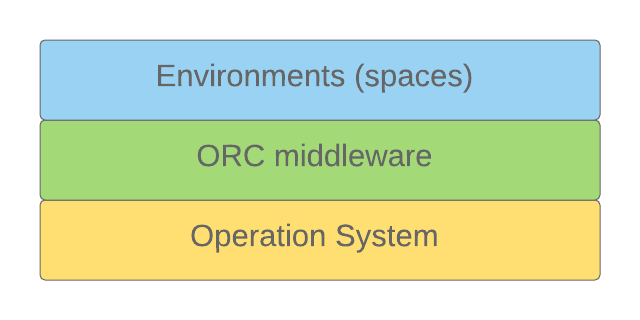
\includegraphics[width=5cm]{os-orc-spaces}
\caption{Octa-node layers}
\end{figure}

Secure channel is implemented using HTTPS\cite{https} protocol with validating each request using security token.

Security token is a fingerprint of the node, it's calculated in the following manner:

\begin{verbatim}
    Token = SHA256(IP, Timestamp, RandomInt)
\end{verbatim}

Where

\begin{itemize}
    \item IP - node public IPv4 address
    \item Timestamp - the time when node is installed in milliseconds
    \item RandomInt - random integer number
\end{itemize}

Commands recieved by the node is executed in the isolated environments.
These environments called \textbf{spaces} and implemented using Docker technology.
\textbf{Spaces} divided into two types: mandatory and task specific

\begin{figure}[h]
\centering
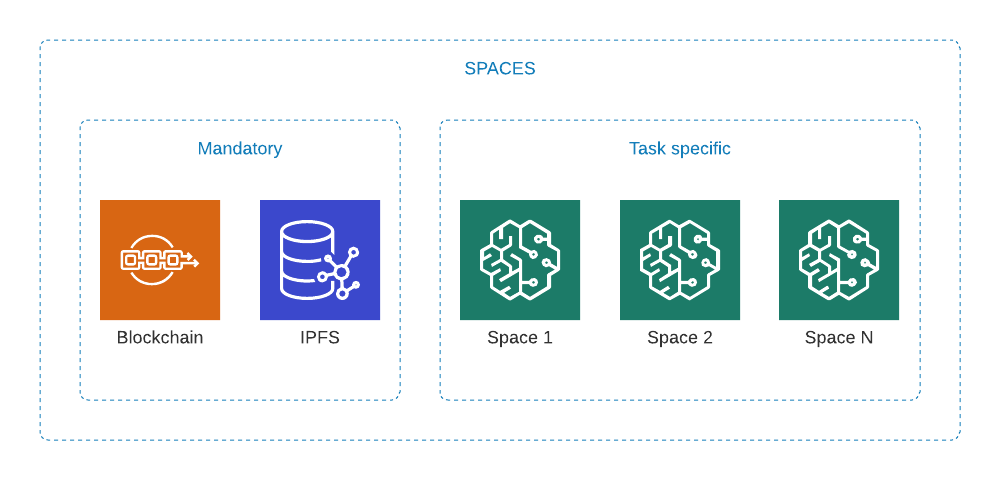
\includegraphics[width=10cm]{spaces}
\caption{Spaces}
\end{figure}

Mandatory \textbf{spaces} are always up and performs network maintainance and support functions.
Task specific \textbf{spaces} running on-demand and depends of type of task which needs to be done.

System data collected by \textbf{ORC}:

\begin{itemize}
    \item CPU information eg. amount, speed and utilization of cores
    \item GPU information including amount and model of GPUs, memory size and amount of graphic processors
    \item Total and free disk space, IO metrics
    \item Total and free memory amount
    \item Performance metrics like request-response time, network latency and so on
\end{itemize}

These data is used to improve the quality of nodes and exclude low performance nodes or non stable ones.

For cases when it's impossible to use IPFS for task data \textbf{ORC} will use internal storage.
